\documentclass{article}
\usepackage{enumerate}
\usepackage{algorithm}
\usepackage{algorithmic} % pesudo code

\usepackage{hyperref}

\usepackage{tikz}
\usetikzlibrary{positioning,shapes,arrows, calc, fit, trees}
\tikzset{
    %Define standard arrow tip
    >=stealth',
    %Define style for boxes
    punkt/.style={
           rectangle,
           rounded corners,
           draw=black, very thick,
           text width=6.5em,
           minimum height=2em,
           text centered},
    % Define arrow style
    pil/.style={
           ->,
           thick,
           shorten <=2pt,
           shorten >=2pt,}
}

\usepackage{amsmath,amsfonts,amsthm} % Math packages
\usepackage{graphicx}
\usepackage{caption}
\usepackage{subcaption}

\usepackage{dcolumn}
\usepackage{booktabs}
\newcolumntype{M}[1]{D{.}{.}{1.#1}}
\newcommand{\norm}[1]{\left\lVert #1 \right\rVert}
\newtheoremstyle{quest}{\topsep}{\topsep}{}{}{\bfseries}{}{ }{\thmname{#1}\thmnote{ #3}.}
\theoremstyle{quest}
\newtheorem*{question}{Question}
\begin{document}
\section*{Propositional Logic}
\begin{enumerate}
\item
Prove or find a counterexample for all 
statements below
\begin{enumerate}[a.]
\item
When P is false, $P\land \neg P$ is false, so $P\land \lnot P$ is not valid.
\item
When B is false and A is false, $A\rightarrow B$ can still be true. Thus $A\rightarrow B \models B$ fails.
\item
\begin{proof}
(A or B) is true, when either A or B is true. When B is true, since $(B\models C)$, C is true. When A is true, since $(A\models B)$, B is true, then C is true.
\qedhere
\end{proof}
\item
\begin{proof}
\begin{align*}
A\lor \lnot (B \land \lnot C) &= A \lor (\lnot B \lor C) \\
& = A \lor C \lor \lnot B 
\end{align*}
$$A \lor C \subseteq A\lor C \lor \lnot B $$
$$A\lor \lnot (B \land \lnot C)  \models A\lor C$$
\qedhere
\end{proof}
\item
When A is false, $\lnot (A\land B) \land (A\rightarrow B)$ is true, thus satisfiable. $(\lnot A \lor \lnot B)\land (\lnot A \lor B)$
\item
No. $((A\rightarrow \lnot B) \land A) = (\lnot A \lor \lnot B) \land A$, there is only one model A is true and B is false can make it true. While $(A\land (B\lor C))$ has more than one model: e.g. A is ture, B is true and C is ture; A is true, B is false, and C is true. 
\end{enumerate}
\end{enumerate}
\section*{First-order Logic}
\begin{enumerate}
\setcounter{enumi}{1}
\item
Translate the following first order logic 
sentences to English. Predicates and functions carry the obvious 
meanings. 
\begin{enumerate}[a.]
\item
Northwestern's mascot is Willie Wildcat.
\item
For any x, y and z, if the sum of x and y is odd and z is odd, then the sum of x, y and z is not odd.
\end{enumerate}
\item
Translate the following English sentences to 
first order logic. Name predicates and functions such that their 
meanings are obvious. 
\begin{enumerate}[a.]
\item
$[student(Greg) \land student(John)]\land play(Greg, tennis)$
\item
$\forall x, \forall y, [integer(x) \land integer(y)] \rightarrow integer(product(x, y))$
\end{enumerate}
\item
Security personnel.
\begin{enumerate}[(i)]
\item
\begin{enumerate}[a.]
\item
$\forall x, [\exists y, P(x) \rightarrow [S(y) \land A(x,y)]]$
\item
$\forall y, [\exists x, S(y) \rightarrow [A(x, y) \land P(x)]]$
\item
$\forall x, [\forall y, A(x,y) \rightarrow M(x,y)]$
\item
$\forall x, \forall y, M(x,y) \rightarrow [O(x) \land O(y)]$
\item
S(Juan)
\item
P(Sarah)
\item
O(Sarah)
\item
A(Sarah, Juan)
\end{enumerate}
\item
Convert to CNF:
\begin{enumerate}[A]
\item
\begin{enumerate}[1]
\item
$\lnot P(x) \lor S(y)$
\item
$\lnot P(x) \lor A(x,y)$
\end{enumerate}
\item
\begin{enumerate}[1]
\item
$\lnot S(y) \lor A(x,y)$
\item
$\lnot S(y) \lor P(x)$
\end{enumerate}
\item
~~~$\lnot A(x, F(x)) \lor M(x, F(x))$
\item
\begin{enumerate}[1]
\item
$\lnot M(x, G(x)) \lor O(x)$
\item
$\lnot M(x, G(x)) \lor O(G(x))$
\end{enumerate}
\item
~~~$S(Juan)$
\item
~~~$P(Sarah)$
\end{enumerate}

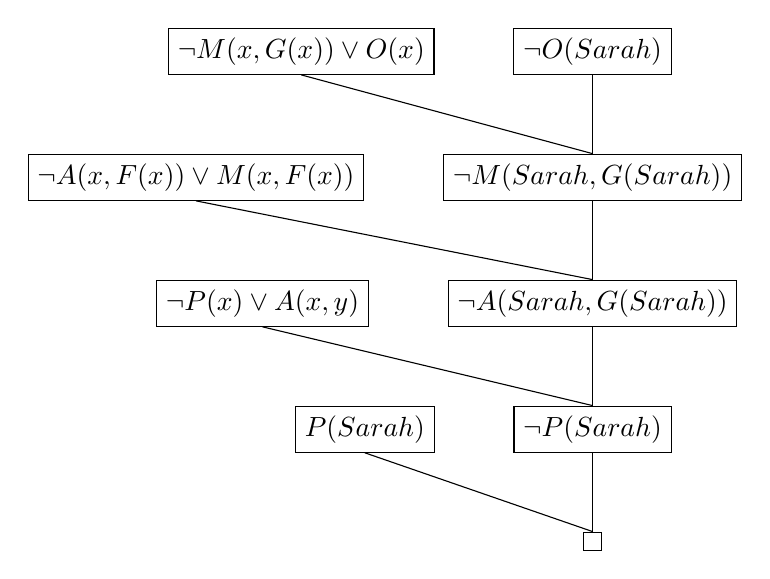
\begin{tikzpicture}
\node[draw, rectangle] (a) {$\lnot M(x, G(x)) \lor O(x)$};
\node[draw, rectangle, right=of a] (b) {$\lnot O(Sarah)$};
\node[draw, rectangle, below=of b] (c) {$\lnot M(Sarah, G(Sarah))$};
\node[draw, rectangle, left=of c] (d) {$\lnot A(x, F(x)) \lor M(x, F(x))$};
\node[draw, rectangle, below=of c] (e) {$\lnot A(Sarah, G(Sarah))$};
\node[draw, rectangle, left=of e] (f) {$\lnot P(x) \lor A(x,y)$};
\node[draw, rectangle, below=of e] (g) {$\lnot P(Sarah)$};
\node[draw, rectangle, left=of g] (h) {$P(Sarah)$};
\node[draw, rectangle, below=of g, minimum height=0.2cm] (i) {};
\draw[-] (b.south) -- (c.north);
\draw[-] (a.south) -- (c.north);
\draw[-] (c.south) -- (e.north);
\draw[-] (d.south) -- (e.north);
\draw[-] (e.south) -- (g.north);
\draw[-] (f.south) -- (g.north);
\draw[-] (g.south) -- (i.north);
\draw[-] (h.south) -- (i.north);
\end{tikzpicture}
\item
The derived clause: $\lnot A(Sarah, G(Sarah))$.

Because we don't know whether there exists advising meeting between Sarah and Juan, i.e. we can't prove M(Sarah, Juan). 
\end{enumerate}
\end{enumerate}
\section*{Bayes Nets}
\begin{enumerate}
\setcounter{enumi}{4}
\item
\begin{enumerate}[a.]
\item
$1+1+2+4+4=12$
\item
$2^5-1 = 31$
\item
ii, vi, vii, ix.
\item
$P(M=1|S)=1/2$

$P(S=1)P(Z=1)P(M=1|S)P(T=1|S,Z)P(A=1|M,T)=1/50$

$\rightarrow P(T=1|S,Z)*P(A=1|M,T)=16/25$

%\centering
\begin{tikzpicture}
\node[draw, circle] (ns) {S};
\node[draw, circle, below left=of ns] (nm) {M};
\node[draw, circle, below right=of ns] (nt) {T};
\node[draw, circle, above right=of nt] (nz) {Z};
\node[draw, circle, below right=of nt] (na) {A};
\node[above=1.75cm of nm] (ts)
{
\begin{tabular}{M{1}M{1}}
\toprule
\multicolumn{2}{c}{S} \\
\multicolumn{1}{c}{T} & \multicolumn{1}{c}{F} \\
\cmidrule{1-2}
0.25 & 0.75 \\
\bottomrule
\end{tabular}
};
\node[right=3.75cm of ts]
{
\begin{tabular}{M{1}M{1}}
\toprule
\multicolumn{2}{c}{Z} \\
\multicolumn{1}{c}{T} & \multicolumn{1}{c}{F} \\
\cmidrule{1-2}
0.25 & 0.75 \\
\bottomrule
\end{tabular}
};
\node[left=0.7cm of nm]
{
\begin{tabular}{cM{1}M{1}}
\toprule
& \multicolumn{2}{c}{M} \\
S & \multicolumn{1}{c}{T} & \multicolumn{1}{c}{F} \\
\cmidrule(r){1-1}\cmidrule(l){2-3}
F & 0.5 & 0.5 \\
T & 0.5 & 0.5 \\
\bottomrule
\end{tabular}
};
\node[right=1.7cm of nt]
{
\begin{tabular}{ccM{2}M{2}}
\toprule
& & \multicolumn{2}{c}{T} \\
\multicolumn{2}{l}{S ~~~Z} & \multicolumn{1}{c}{T} & \multicolumn{1}{c}{F} \\
\cmidrule(r){1-2}\cmidrule(l){3-4}
F & F & 0.8 & 0.2 \\
F & T & 0.8 & 0.2 \\
T & F & 0.8 & 0.2 \\
T & T & 0.8 & 0.2 \\
\bottomrule
\end{tabular}
};
\node[below=1cm of nm]
{
\begin{tabular}{ccM{2}M{2}}
\toprule
& & \multicolumn{2}{c}{A} \\
\multicolumn{2}{l}{M ~~~T} & \multicolumn{1}{c}{T} & \multicolumn{1}{c}{F} \\
\cmidrule(r){1-2}\cmidrule(l){3-4}
F & F & 0.8 & 0.2 \\
F & T & 0.8 & 0.2 \\
T & F & 0.8 & 0.2 \\
T & T & 0.8 & 0.2 \\
\bottomrule
\end{tabular}
};
\path (ns) edge[-latex] (nm)
(ns) edge[-latex] (nt) 
(nz) edge[-latex] (nt)
(nm) edge[-latex] (na)
(nt) edge[-latex] (na);
\end{tikzpicture}
\item
9.
\end{enumerate}
\end{enumerate}
\end{document}
